\documentclass{article}
\usepackage{spconf,amsmath,graphicx,hyperref}
\usepackage{amsmath}
\usepackage[flushleft]{threeparttable}
\usepackage{cite}
\usepackage{booktabs, multirow}
\usepackage{enumitem} %缩进itemize
\usepackage{amssymb}
\usepackage{xcolor}

\newif\ifshowchanges
\showchangestrue
% \showchangesfalse
\newcommand{\rev}[1]{%
  \ifshowchanges
    \textcolor{red}{#1}%
  \else
    #1%
  \fi
}
\usepackage[table]{xcolor}
\usepackage{pgf}

\definecolor{heatblue}{RGB}{65,115,200}
\definecolor{heatred}{RGB}{205,92,92}

\newcommand{\heatpos}[1]{%
  \pgfmathtruncatemacro{\shadevalue}
    {min(54,14+40*sqrt((#1)/10))}%
  \edef\heatcolor{heatblue!\shadevalue}%
  \expandafter\cellcolor\expandafter{\heatcolor}%
  $+$#1%
}

\newcommand{\heatneg}[1]{%
  \pgfmathtruncatemacro{\shadevalue}
    {min(54,14+40*sqrt((#1)/10))}%
  \edef\heatcolor{heatred!\shadevalue}%
  \expandafter\cellcolor\expandafter{\heatcolor}%
  $-$#1%
}

\newcommand{\heatposbest}[1]{%
  \pgfmathtruncatemacro{\shadevalue}
    {min(54,14+40*sqrt((#1)/10))}%
  \edef\heatcolor{heatblue!\shadevalue}%
  \expandafter\cellcolor\expandafter{\heatcolor}%
  $\mathbf{+}$\textbf{#1}%
}

\newcommand{\heatnegbest}[1]{%
  \pgfmathtruncatemacro{\shadevalue}
    {min(54,14+40*sqrt((#1)/10))}%
  \edef\heatcolor{heatred!\shadevalue}%
  \expandafter\cellcolor\expandafter{\heatcolor}%
  $\mathbf{-}$\textbf{#1}%
}

% \usepackage{lilyglyphs} % dynamic symbols
% \usepackage{tikz}
% \usetikzlibrary{arrows.meta,positioning,fit,calc}
% \tikzset{
%   block/.style={draw, rounded corners, very thick, align=center, inner sep=3pt, minimum height=8mm, fill=white},
%   tinyblock/.style={draw, rounded corners, thick, inner sep=2pt, minimum height=4mm, fill=white},
%   arrow/.style={-Latex, very thick}
% }

% \title{CASM: A Context-Aware Semi-Markov Alternative to DBN Post-Processor for Beat Tracking}

\title{CASM: Context-Aware Semi-Markov Post-Processor for Beat Tracking}

\name{Zhanhong He$^{1,2}$, Hanyu Meng$^{1,3}$, Yaolong Ju$^{1,}$\sthanks{Corresponding author, juyaolong@gbu.edu.cn.}}
\address{
    $^{1}$Great Bay University, Dongguan, China\\
    $^{2}$The University of Western Australia, Perth, Australia\\
    $^{3}$The University of New South Wales, Sydney, Australia
}

\begin{document}
\ninept
\maketitle

\begin{abstract}
At the final stage of music beat tracking, neural activations need to be decoded into a discrete, musically coherent event sequence. Direct peak picking follows the local evidence but tends to produce spurious and missed detections. Dynamic Bayesian networks (DBNs), the dominant post-processing approach, suppress such errors by imposing explicit human-specified global assumptions. They work well when predefined tempo and meter assumptions match the music, but expressive or rhythmically complex pieces often depart from them, resulting in overrides correct local evidence instead of correcting it. We address this limitation by proposing CASM, a model-agnostic, context-aware semi-Markov decoder that exploits local structure in beat activations. CASM estimates local periodicity and ambiguity from the activations, then commits strongly when the cues are clear and relaxes toward the neural output when they are ambiguous, with built-in safeguards keeping this behavior stable and predictable. Using a single configuration, CASM improves F1, CMLt, and AMLt across BeatThis, MSCNN, and TCN models on GTZAN, and delivers state-of-the-art performance on SMC. Further analysis shows that CASM is less sensitive than DBNs to the choice of calibration data.\footnote{Code and demo are available at \url{https://zhanh-he.github.io/casm-beat-tracking}.}
\end{abstract}

\begin{keywords}
beat tracking, context-aware, semi-Markov model, post-processing, local periodicity
\end{keywords}

\section{Introduction}
\label{sec:intro}
Beats give music its temporal scaffold, so reliable beat tracking is crucial for music production, analysis, synchronization, and interactive systems~\cite{purwins2019deep}. More recently, beat tracking has become a key component of multimodal AI-generated content (AIGC), where the estimated beats serve as timing anchors for aligning generated content such as dance~\cite{tseng2023edge, huang2024beatit}, video~\cite{yu2023loris, tong2026vem}, and music~\cite{lan2024musicongen, chen2024musicldm}. Most music beat trackers operate in two stages: a network maps audio to framewise beat activations, and a post-processor converts these activations into discrete events. Despite recent attempts to remove the post-processor~\cite{chen2022postprocessingfree, foscarin2024beat, bolt2026reformulated}, many contemporary systems \cite{deng2024efficient, ru2025hingenet, ru2025beatfm, ru2026beatmamba, zhang2025beatkan} still rely on it to obtain musically coherent estimates. However accurate the neural activations become, direct peak picking makes isolated local decisions without considering the periodicity of beat sequences. Post-processing addresses this limitation by combining local activation evidence with the temporal regularity of music.

For post-processors, the key design question is how to balance temporal regularity against local activation evidence. A weak regularity constraint preserves the network's predictions but may fail to correct missed or spurious beats, whereas an overly strong one may suppress correct activation peaks in passages with expressive
timing or frequent local tempo changes, as is common in classical music performances~\cite{Schreiber2020LocalTempo}. 

Many existing post-processors tilt this balance toward predefined temporal constraints. Early dynamic programming approach~\cite{ellis2007beattracking} assumes a single global tempo per track and penalizes inter-beat intervals (IBIs) that deviate from it. Conditional random fields (CRFs)~\cite{fillon2015crf, fuentes2019skipchain} learn sequence preferences that permit a range of local tempo variation while discouraging abrupt IBI changes. The dominant post-processor is the dynamic Bayesian network (DBN)~\cite{krebs2015dbn, bock2016joint}, which operates under pre-specified tempo ranges, meter states, and tempo transition probabilities. This design works well when these assumptions match the recording, but may require per-track or corpus-specific retuning when they do not~\cite{ahn2026smcblindspot}.

The recently proposed PLPDP~\cite{chiu2023localperiodicity} shifts this balance by letting local evidence shape the temporal constraint. It derives a time-varying IBI and confidence from the predominant local pulse (PLP), which set the preferred period and how strongly it is enforced. However, this confidence is derived from PLP peak heights, it reflects how strong the selected period is but not whether a competing period is nearly as plausible. A strong period may still be nearly tied with a metrical alternative, such as half or double tempo, and enforcing it strongly then risks committing to the wrong metrical level.

\begin{figure*}[h!]
\centering
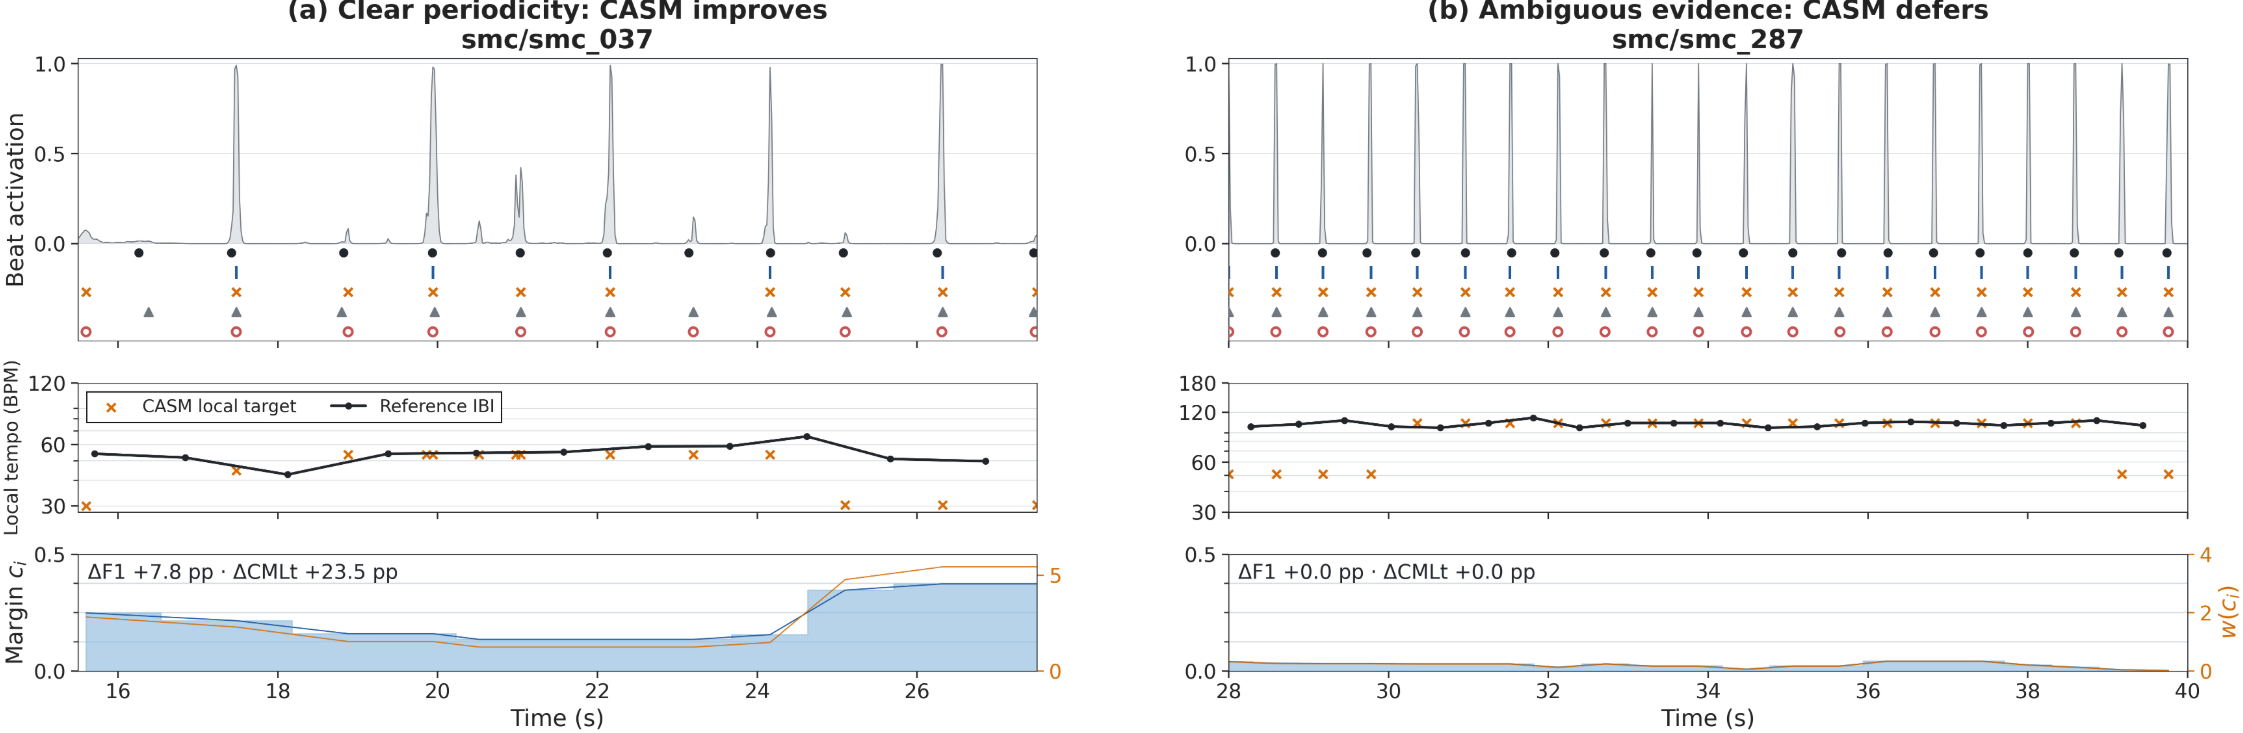
\includegraphics[width=0.9\textwidth]{figures/p0.jpg}
\caption{CASM behaviour on held-out Beat This activations from SMC. Clear local periodicity recovers weak activation-supported beats (left), whereas ambiguous competing periods make CASM defer to Direct (right). Reference IBI is shown only for interpretation.}
\label{fig:casm-examples}
\end{figure*}

We introduce CASM, a context-aware semi-Markov post-processor. The core philosophy of our approach is simple: whereas PLPDP measures periodicity strength, CASM additionally considers periodicity ambiguity. By constructing a sparse path over activation-supported peaks, CASM explicitly estimates both factors. When periodic evidence is unambiguous, CASM enforces strict temporal regularity. When competing periods create ambiguity, it weakens the temporal constraint and allows the neural activations to dominate. Bounded by a beat-count safeguard and a beat-synchronous meter decoder for deterministic performance, CASM offers four core advantages:
\begin{itemize}[leftmargin=*, nosep]
\item \textbf{Model-agnostic.} CASM is a plug-in post-processor that operates on existing beat tracking systems and requires no neural network retraining.
\item \textbf{Low tuning burden.} CASM derives its temporal constraint directly from the activations like PLPDP, requiring less per-track or per-dataset tuning than DBNs.
\item \textbf{Good generalization.} By evaluating periodicity ambiguity, a single CASM configuration robustly handles both steady and complex rhythms across the MIREX2026 benchmark evaluation datasets: GTZAN (common genres) and SMC (deliberately challenging).
\item \textbf{Open and ready to use.} We release CASM as an open-source, pip-installable package with an interface compatible with the DBN post-processors in \textit{madmom}.
\end{itemize}


% We introduce CASM, a context-aware semi-Markov post-processor. Whereas PLPDP measures periodicity strength, CASM additionally considers periodicity ambiguity. CASM constructs a sparse path over activation-supported peaks and estimates both the local periodicity and its ambiguity, which together control the target, strength, and tolerance of the segment-duration preference. When the periodic evidence is clear, CASM commits strongly to local regularity and can recover weak but activation-supported beats that direct peak picking misses; when competing periods are similarly plausible, it weakens this preference and lets the neural activations dominate. A beat-count safeguard and a beat-synchronous meter decoder further keep the procedure deterministic and predictable. The core advantages of CASM are as follows:




\section{Methodology}
\label{sec:method}

\subsection{CASM Overview}
The proposed Context-Aware Semi-Markov (CASM) decoder is a model-agnostic post-processor that operates on beat and downbeat activations produced by a frozen tracker. It modifies only the decoding stage and therefore requires no retraining. Like PLPDP, CASM estimates a local beat period and its support from the activation sequence. CASM differs in how this support is defined and used: it measures the separation between the dominant period and competing tempo hypotheses and uses this margin to adapt the rhythmic constraint. Consequently, CASM enforces local regularity when the periodic evidence is clear, but relaxes the constraint when the evidence is ambiguous.



\subsection{Context-aware beat decoding}
A frozen tracker produces a beat logit $z_t^{\mathrm b}$ at each
frame $t$, with activation $a_t=\operatorname{sigmoid}(z_t^{\mathrm b})$ and frame rate $F$. We retain local maxima above a fixed threshold $\theta_{\mathrm c}$ as candidates $\mathcal C=\{t_1,\ldots,t_N\}$, assigning each candidate a clipped evidence score $e_i$. For $i<j$, the elapsed time is
$\Delta_{ij}=(t_j-t_i)/F$, and edge $(i,j)$ is admissible when
$60/\Delta_{ij}$ lies within 30--300 BPM. CASM selects an ordered candidate path
$\pi=(i_1,\ldots,i_K)$, with $i_1<\cdots<i_K$, by maximizing

\begin{equation}
\mathcal S(\pi)
=
\sum_{k=1}^{K} e_{i_k}
-
\sum_{k=2}^{K}D_{i_{k-1},i_k}
\label{eq:casm-objective}
\end{equation}
where $D_{ij}$ is the duration cost between candidates $i$ and $j$.
The two terms respectively reward strong beat evidence and penalize
rhythmically inconsistent intervals. Because each transition scores a
variable-duration interval, CASM has a semi-Markov structure.

At candidate $i$, $q_i(\ell)$ denotes the normalized
autocorrelation score at an admissible lag $\ell$ within a window
centred on $t_i$, including a mild fast-tempo prior. The dominant lag
$\ell_i^\star=\arg\max_\ell q_i(\ell)$ gives the local period
$\tau_i=\ell_i^\star/F$. We define the strongest competing hypothesis
outside a $\pm2$-frame neighbourhood as
$q_i^{\mathrm{alt}}
=\max_{\ell:\,|\ell-\ell_i^\star|>2}q_i(\ell)$.
The normalized period-separation margin is

\begin{equation}
c_i =
\operatorname{clip}_{[0,1]}\!\left(
\frac{
q_i(\ell_i^\star)-q_i^{\mathrm{alt}}
}{
|q_i(\ell_i^\star)|+\epsilon_c
}
\right)
\label{eq:casm-reliability}
\end{equation}

where $\epsilon_c>0$ stabilizes the denominator. A large $c_i$
indicates a clearly dominant period, whereas a small value indicates
ambiguity, including half- or double-time alternatives. Thus, $c_i$ is a deterministic separation margin rather than a calibrated
probability. Both $\tau_i$ and $c_i$ are median-filtered over five
consecutive candidates.

For edge $(i,j)$, CASM combines the endpoint estimates as
$\bar{\tau}_{ij}=\sqrt{\tau_i\tau_j}$ and
$c_{ij}=\sqrt{c_i c_j}$. The ambiguity-conditioned constraint strength
is
$g(c)=\lambda c/\{2[\sigma_0+(1-c)\sigma_{\mathrm u}]^2\}$,
giving the duration cost

\begin{equation}
D_{ij}
=
g(c_{ij})\,
\log^2\!\left(
\frac{\Delta_{ij}}{\bar{\tau}_{ij}}
\right)
\label{eq:casm-duration}
\end{equation}

Here, $\lambda>0$ controls the overall penalty strength,
$\sigma_0>0$ sets the minimum timing tolerance, and
$\sigma_{\mathrm u}\geq0$ controls relaxation under ambiguity.
The cost vanishes when $\Delta_{ij}=\bar{\tau}_{ij}$; a large $c_{ij}$
enforces rhythmic regularity, while a small $c_{ij}$ relaxes the
constraint. CASM can therefore recover weak but rhythmically supported beats without forcing an unreliable tempo grid.

% \begin{figure}[!h]
% \centering
% 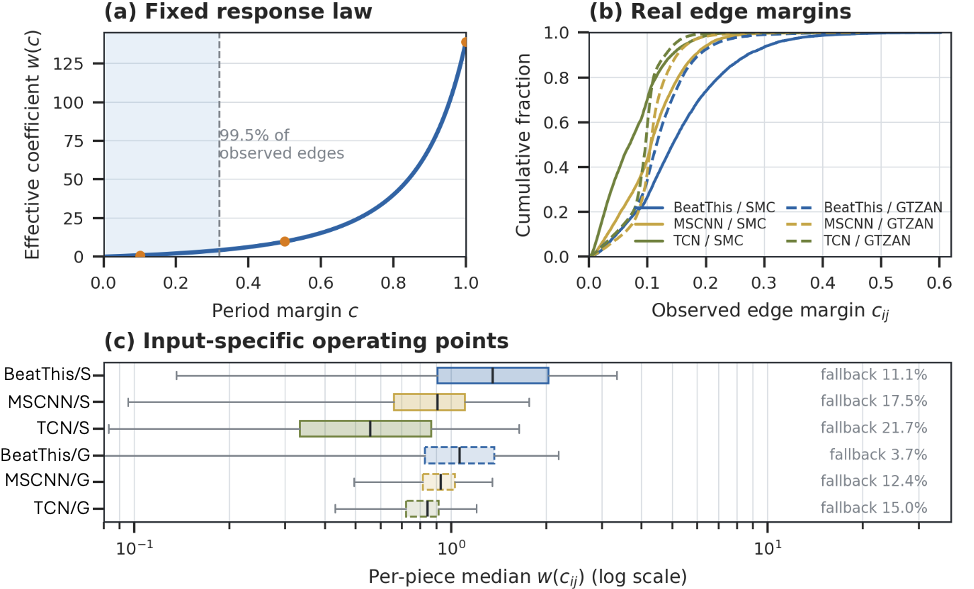
\includegraphics[width=\columnwidth]{figures/p1.jpg}
% \caption{Input-conditioned duration stiffness under one frozen CASM
% configuration. (a) The fixed constants map period margin $c$ to coefficient $w(c)$; shading contains 99.5\% of observed structured-path edges. (b) Edge margin distributions differ across backbones and corpora. (c) Per-piece median coefficients therefore occupy different operating ranges; annotations give the separate count-ratio fallback rate. Fixed parameters define one response law, not one effective rigidity for every input.}
% \label{fig:casm-response}
% \end{figure}

Figure~\ref{fig:casm-response} shows how Eq.~\eqref{eq:casm-duration} converts the local period-separation margin into an input-dependent timing constraint. Panel (a) shows the fixed response, panel (b) maps transitions from different datasets and backbones onto it, and panel (c) summarizes the resulting track-level
constraint strengths. Thus, one frozen CASM configuration adapts its
constraint across inputs. The figure illustrates decoder conditioning,
not tracking accuracy; the direct fallback is a separate safeguard.

\subsection{Safeguards and downbeat decoding}
A Viterbi-style dynamic program maximizes
Eq.~\eqref{eq:casm-objective} and backtracks the best beat path, allowing
a restart after an unfavourable prefix. As a safeguard, CASM also forms
a direct fallback path using seven-frame max pooling, a zero-logit
threshold, and one-frame deduplication
\cite{foscarin2024beat}. If
$\lvert\pi_{\mathrm{CASM}}\rvert/
 \lvert\pi_{\mathrm{direct}}\rvert
 \notin[r_{\min},r_{\max}]$,
indicating an implausibly sparse or dense CASM path, the direct path is returned. This rule is deterministic and requires no learned router.

Downbeats are decoded on the selected beat grid using a second
dynamic program that favours valid bar lengths and discourages
unnecessary meter changes. If its output strongly disagrees with the
direct downbeat activations snapped to the same grid, the snapped result is used, ensuring that every downbeat coincides with an output beat. All scalar parameters are calibrated once on the development folds and then frozen across tracks, datasets, and backbone models. Inference
requires no reference annotations, externally supplied BPM or meter,
per-track tuning, or learned decoder parameters.

\section{Experiments}\label{sec:exp}

\subsection{Evaluation protocol}
\textbf{Datasets and splits.} We use the publicly released data from BeatThis \cite{foscarin2024beat}, which contains 4,556 tracks from 18 beat-tracking datasets, including SMC, Hainsworth, Ballroom, Beatles, and others. This data collection provides preprocessed log-Mel spectrograms computed from 22.05kHz mono audio at 50 fps, together with a fixed eight-fold partition to conduct cross-validation experiments. For each fold, the corresponding backbone checkpoint is trained on the remaining seven folds, ensuring that evaluated tracks remain unseen during training. Among these datasets, SMC provides beat but not downbeat annotations, and is widely recognized as the hard one compared to the others. Additionally, GTZAN provides 993 tracks as the held-out evaluation set, which is excluded from the cross-validation pool.

\textbf{Backbones.} We select three models whose implementations are publicly available and readily reproducible. For BeatThis, we use the original code and pretrained checkpoints \cite{foscarin2024beat}. MSCNN is adapted from the multi-scale, multi-task convolutional network of \cite{he2026dynest}, which was designed for 60s Bark-scale specific-loudness features. We modify it to accept the 30s the unified log-Mel input and remove the task heads unrelated to beat and downbeat tracking. TCN was introduced by \cite{bock2020deconstruct}, and we use the re-implementation distributed with \cite{he2026dynest}, which has been adapted from its original 5\,s input to the same 30\,s log-Mel input, with the tempo task head removed. All resulting backbones are trained on the same data and frozen before decoding performance comparison, ensuring that every post-processor receives exactly the same 50\,Hz framewise beat/downbeat activations from a given backbone.

\textbf{Evaluation.} We conduct the same eight-fold cross-validation as in \cite{foscarin2024beat}, where backbones are each evaluated on the held-out GTZAN and their corresponding out-of-fold SMC partitions. We use \texttt{mir\_eval} \cite{raffel2014mireval} to compute F1 score with a $\pm70$\,ms tolerance, CMLt, and AMLt. CMLt measures continuity at the correct metrical level, whereas AMLt additionally accepts standard off-beat and half- or double-level interpretations.

%CombFilter \cite{bock2015combfilter}, 

\subsection{Post-processors and tempo support}
As we defined our task is offline, the future information is accessible for model to top up the estimate accuracy. We compare CASM with the direct decoding, along with other offline post-processing methods including DBN \cite{krebs2015dbn}, PLPDP \cite{chiu2023localperiodicity}, and CRF beat detection \cite{korzeniowski2014crf}. Direct is the peak-picking path defined in Sec.~\ref{sec:method}, and CASM uses its fixed 30--300-BPM support. PLPDP, CombFilter, and CRF are run with their released/default parameters. For methods without a joint beat/downbeat decoder, downbeats are decoded from the downbeat activation stream and snapped to the corresponding beat grid.

DBN receives separate treatment because its behaviour is particularly sensitive to global tempo support. We use the standard joint \texttt{madmom} configuration \cite{krebs2015dbn}: meters $\{3,4\}$, transition weight 100, observation weight 16, threshold 0.05, and the default 55--215-BPM range. Since many SMC data are fall below 55 BPM \cite{ahn2026smcblindspot}, Table~\ref{tab:postprocessor_ablation} also explores a 30--300-BPM DBN variant in which only the tempo range is changed. For a matched diagnostic, we additionally report CASM with its support restricted to 55--215 BPM on BeatThis activations, with all other CASM settings remain unchanged.

\subsection{CASM calibration}
CASM has no learned weights or random seed. The final configuration used in all main tables is calibrated once on the union of SMC folds 1--7 (7F) and then frozen for every track, backbone, and dataset. The same global scalar settings are therefore used on BeatThis, MSCNN, and TCN, on both SMC and GTZAN, without per-track or per-dataset BPM, meter, or parameter tuning at inference. Because the aggregate SMC results use eight-fold out-of-fold backbone activations while the decoder configuration is calibrated on folds 1--7, they are out-of-fold with respect to backbone training but are not a nested estimate of decoder calibration.

We analyse calibration-data sensitivity separately rather than using it to choose the main operating point. SMC fold 0 is held out from decoder calibration throughout. From folds 1--7, we enumerate every 1-, 2-, and 4-fold calibration subset ($7$, $21$, and $35$ combinations) and the seven-fold union. For both CASM and DBN, a decoder configuration is selected independently on each calibration subset and then evaluated on the same fixed SMC-fold-0 panel and on GTZAN using one fixed backbone seed. The resulting distributions therefore measure sensitivity to the amount and composition of calibration data, while the 7F CASM configuration is the maximally supported global configuration used for the main results.


\section{Results}
\label{sec:results}

\subsection{Comparison with post-processors}
Table~\ref{tab:postprocessor_ablation} isolates the post-processor by holding the backbone activations fixed. With 30--300-BPM support, the CASM improves BeatThis (compared with direct pick-peaking) on every reported metrics across all three backbones and both datasets. Relative to DBN, CASM generally preserves F1 better, while DBN can produce larger continuity gains, particularly for GTZAN downbeats. The large SMC change between the 55--215- and 30--300-BPM DBN variants also shows how strongly a fixed DBN can depend on its global tempo range. PLPDP, CombFilter, and CRF provide useful alternatives, but none improves every reported metric under the same fixed activations. Overall, CASM gives a conservative F1--continuity operating point that transfers across backbone families without changing decoder parameters.

\begin{table}[!h]
\centering
\caption{Post-processing comparison on fixed backbone activations. Backbone-only rows use direct peak picking. Post-processors use 30--300 BPM unless marked $^{\mathrm{[dbn]}}$, which denotes the 55--215 BPM range optimized for DBN in GTZAN-like music.}
\label{tab:postprocessor_ablation}
\begingroup
\fontsize{8pt}{8.5pt}\selectfont
\setlength{\tabcolsep}{0.3pt}
\renewcommand{\arraystretch}{0.92}
\resizebox{\columnwidth}{!}{%
\begin{tabular}{l|rrr@{\hspace{2pt}}|rrr@{\hspace{2pt}}|rrr}
\toprule
\multicolumn{1}{c|}{\multirow{2}{*}{\textbf{Method}}}
& \multicolumn{6}{c|}{\textbf{GTZAN (Beat / Downbeat)}}
& \multicolumn{3}{c}{\textbf{SMC (Beat)}} \\
\cmidrule(lr){2-7}
\cmidrule(l){8-10}
& F1 & CMLt & AMLt
& F1 & CMLt & AMLt
& F1 & CMLt & AMLt \\
\midrule
\textbf{BeatThis}(direct)\cite{foscarin2024beat}
& 89.1 & 79.8 & 89.8
& 78.3 & 67.2 & 79.1
& 62.7 & 51.4 & 61.0 \\
w. CASM
& \heatposbest{0.3} & \heatposbest{0.8} & \heatpos{1.2}
& \heatposbest{0.7} & \heatpos{3.6} & \heatpos{8.0}
& \heatposbest{0.3} & \heatposbest{2.4} & \heatposbest{3.6} \\
% w. CASM$^{\mathrm{[dbn]}}$
% & \heatpos{0.1} & \heatpos{0.5} & \heatpos{0.6}
% & \heatpos{0.5} & \heatpos{2.9} & \heatpos{5.8}
% & \heatpos{0.1} & \heatpos{0.4} & \heatpos{2.0} \\
w. DBN \cite{krebs2015dbn}
& \heatneg{0.5} & \heatneg{0.9} & \heatpos{0.2}
& \heatneg{1.5} & \heatneg{0.6} & \heatpos{1.1}
& \heatneg{1.6} & \heatpos{0.4} & \heatpos{3.5} \\
w. DBN$^{\mathrm{[dbn]}}$
& \heatneg{1.0} & \heatpos{0.7} & \heatpos{1.3}
& \heatneg{0.9} & \heatposbest{6.2} & \heatposbest{8.7}
& \heatneg{5.2} & \heatneg{3.9} & \heatpos{1.5} \\
w. PLPDP \cite{chiu2023localperiodicity} \space{}
& \heatpos{0.1} & \heatpos{0.3} & \heatpos{0.3}
& \heatpos{0.1} & \heatpos{0.2} & \heatpos{0.2}
& \heatneg{0.9} & \heatneg{3.5} & \heatneg{0.3} \\
w. CRF \cite{korzeniowski2014crf}
& \heatneg{0.6} & \heatneg{0.3} & \heatposbest{1.4}
& \heatneg{1.4} & \heatpos{1.9} & \heatpos{5.5}
& \heatneg{1.2} & \heatpos{1.4} & \heatpos{1.2} \\
\midrule
\textbf{MSCNN}\cite{he2026dynest}
& 86.1 & 73.4 & 79.9
& 70.8 & 53.1 & 63.1
& 57.2 & 42.0 & 48.4 \\
w. CASM
& \heatposbest{0.4} & \heatpos{1.6} & \heatpos{2.4}
& \heatpos{1.5} & \heatpos{12.5} & \heatpos{18.3}
& \heatposbest{0.3} & \heatposbest{3.5} & \heatposbest{6.8} \\
% w. CASM$^{\mathrm{[dbn]}}$
% &&&
% &&&
% &&& \\
w. DBN
& \heatneg{1.1} & \heatpos{0.2} & \heatpos{5.9}
& \heatneg{0.9} & \heatpos{9.5} & \heatpos{14.6}
& \heatneg{0.2} & \heatpos{2.2} & \heatpos{4.1} \\
w. DBN$^{\mathrm{[dbn]}}$
& \heatneg{0.6} & \heatposbest{4.0} & \heatposbest{7.2}
& \heatposbest{1.8} & \heatposbest{15.8} & \heatposbest{21.2}
& \heatneg{4.9} & \heatpos{0.3} & \heatpos{3.9} \\
\midrule
\textbf{TCN}\cite{bock2020deconstruct}
& 87.1 & 73.8 & 81.7
& 62.4 & 24.6 & 59.9
& 52.9 & 30.1 & 36.0 \\
w. CASM
& \heatposbest{0.3} & \heatposbest{1.3} & \heatpos{1.6}
& \heatpos{2.1} & \heatpos{9.2} & \heatpos{13.4}
& \heatposbest{1.7} & \heatposbest{4.5} & \heatposbest{8.2} \\
% w. CASM$^{\mathrm{[dbn]}}$
% &&&
% &&&
% &&& \\
w. DBN
& \heatneg{1.9} & \heatneg{0.8} & \heatpos{4.4}
& \heatneg{0.2} & \heatpos{8.9} & \heatpos{9.3}
& \heatneg{0.4} & \heatpos{2.1} & \heatpos{5.9} \\
w. DBN$^{\mathrm{[dbn]}}$
& \heatneg{2.6} & \heatneg{0.7} & \heatposbest{5.0}
& \heatposbest{4.9} & \heatposbest{23.2} & \heatposbest{22.9}
& \heatneg{0.9} & \heatneg{7.0} & \heatpos{2.3} \\
\bottomrule
\end{tabular}%
}
\endgroup
\end{table}

\subsection{Ablation study}
Table~\ref{tab:casm_ablation} shows that the main CASM components contribute to a balanced F1--continuity trade-off. Fixing the local-target precision substantially reduces the gains, particularly on GTZAN, while using only periodicity strength or width also degrades Beat F1 and weakens continuity improvements. This supports combining complementary local periodicity cues rather than relying on a single confidence measure. Using one endpoint produces results close to the full CASM, suggesting that this design choice has a relatively small effect. Removing the safeguards can yield slightly larger CMLt or AMLt gains, but at the cost of Beat F1, most clearly on SMC ($+0.2$ to $-0.3$). Overall, the full CASM provides the most consistent balance between preserving local beat evidence and improving temporal continuity across both datasets.

\begin{table}[!h]
\centering
\caption{Ablation study of CASM on BeatThis activations. All values are changes relative to the direct backbone output.}
\label{tab:casm_ablation}
\begingroup
\fontsize{9pt}{10pt}\selectfont
\setlength{\tabcolsep}{3.6pt}
\renewcommand{\arraystretch}{0.95}
\resizebox{\columnwidth}{!}{%
\begin{tabular}{l|rrr@{\hspace{2pt}}|rrr}
\toprule
\multicolumn{1}{c|}{\multirow{2}{*}{\textbf{Method}}}
& \multicolumn{3}{c|}{\textbf{GTZAN (Beat)}}
& \multicolumn{3}{c}{\textbf{SMC (Beat)}} \\
\cmidrule(lr){2-4}
\cmidrule(l){5-7}
& F1 & CMLt & AMLt
& F1 & CMLt & AMLt \\
\midrule
\textbf{CASM} (default, 30--300 BPM)
& \heatposbest{0.3} & \heatposbest{0.8} & \heatposbest{1.2}
& \heatposbest{0.3} & \heatposbest{2.4} & \heatposbest{3.6} \\
Change to 55--215 BPM
& \heatpos{0.1} & \heatpos{0.5} & \heatpos{0.6}
& \heatpos{0.1} & \heatpos{0.4} & \heatpos{2.0} \\
Local target fixed precision
& \heatneg{0.3} & \heatneg{0.8} & \heatneg{0.8}
& \heatpos{0.1} & \heatpos{0.7} & \heatpos{0.9} \\
Strength only
& \heatneg{0.1} & \heatneg{0.2} & \heatneg{0.2}
& \heatneg{0.5} & \heatpos{0.9} & \heatpos{2.1} \\
Width only
& \heatneg{0.3} & \heatneg{0.6} & \heatneg{0.6}
& \heatneg{0.5} & \heatpos{0.9} & \heatpos{2.2} \\
One endpoint
& \heatpos{0.1} & \heatpos{0.3} & \heatpos{0.4}
& \heatpos{0.2} & \heatpos{2.2} & \heatpos{2.6} \\
No safeguards
& \heatneg{0.1} & \heatpos{0.4} & \heatpos{0.5}
& \heatneg{0.3} & \heatpos{2.5} & \heatpos{2.7} \\
\bottomrule
\end{tabular}%
}
\endgroup
\end{table}


\subsection{Comparison with the state of the art}
Table~\ref{tab:audiodyn_cross_dataset_sota} compares the BeatThis works with CASM results with recent literature. While using CASM improves six beat/downbeat metrics compared to BeatThis (directly peak-picking) on the GTZAN, we reported the highest scores on SMC compared to the other SOTA systems. On GTZAN, stronger task-specific or pre-trained frontends retain the best individual scores. The literature table therefore provides system-level context; controlled claims about decoder behaviour come from Table~\ref{tab:postprocessor_ablation}, where the backbone activations are held fixed.

\begin{table}[!h]
\centering
\caption{Comparison with recent beat-tracking systems. BeatThis (direct) and CASM results were obtained from our experiments, while all other values are reported from their original papers.}
\label{tab:audiodyn_cross_dataset_sota}
\begingroup
\fontsize{9pt}{10pt}\selectfont
\setlength{\tabcolsep}{0.5pt}
\renewcommand{\arraystretch}{1.0}
\resizebox{\columnwidth}{!}{%
\begin{tabular}{l|ccc|ccc|ccc}
\toprule
\multicolumn{1}{c|}{\multirow{2}{*}{\textbf{Method}}}
& \multicolumn{6}{c|}{\textbf{GTZAN (Beat / Downbeat)}}
& \multicolumn{3}{c}{\textbf{SMC (Beat)}} \\
\cmidrule(lr){2-4}
\cmidrule(lr){5-7}
\cmidrule(l){8-10}
& F1 & CMLt & AMLt
& F1 & CMLt & AMLt
& F1 & CMLt & AMLt \\
\midrule
\rowcolor{gray!10}
\textbf{HN-MERT} w.DBN \cite{ru2025hingenet}
& \textbf{89.7} & 81.4 & \textbf{94.3}
& 77.4 & 71.6 & 87.2
& 61.7 & -- & -- \\
\textbf{HN-MusicFM} w.DBN
& 89.2 & 80.9 & 93.7
& \textbf{79.8} & 73.2 & \textbf{89.5}
& 60.6 & -- & -- \\
\rowcolor{gray!10}
\textbf{BeatFM-MERT} w.DBN \cite{ru2025beatfm}
& \underline{89.5} & \underline{82.7} & \underline{93.9}
& 76.7 & 70.2 & 85.4
& 61.3 & -- & -- \\
\textbf{BeatFM-MusicFM} w.DBN
& 89.1 & 80.6 & 93.5
& \underline{79.6} & \underline{74.4} & \underline{88.7}
& 60.5 & -- & -- \\
% \textbf{SpecTNT-TCN} w.DBN \cite{hung2022modeling}
% & 88.7 & 81.2 & 92.0
% & 75.6 & 71.5 & 88.1
% & 60.5 & 51.4 & 66.3 \\
% \textbf{TCN} + DBN  \cite{bock2020deconstruct}
% & 88.5 & 81.3 & 93.1
% & 67.2 & 64.0 & 83.2
% & 55.2 & 46.5 & 64.3 \\
\rowcolor{gray!10}
\textbf{BeatMamba} w.DBN \cite{ru2026beatmamba}
& 88.9 & 82.3 & \textbf{94.3}
& -- & -- & --
& 58.7 & 46.8 & 62.4 \\
\textbf{BeatKAN} w.DBN \cite{zhang2025beatkan}
& 88.2 & 78.1 & 92.3
& -- & -- & --
& 59.8 & 48.4 & 64.0 \\
\rowcolor{gray!10}
\textbf{BeatThis-MDM} \cite{foscarin2026masked}
& \textbf{89.7} & \textbf{82.9} & 92.5
& 79.5 & \textbf{76.4} & 88.5
& 61.0 & 48.9 & \underline{64.3} \\
\midrule
\textbf{BeatThis} \cite{foscarin2024beat}
& 89.1 & 79.8 & 89.8
& 78.3 & 67.2 & 79.1
& \underline{62.7} & \underline{51.4} & 61.0 \\
% \textbf{BeatThis} w.DBN (default \& opt)
% & 88.1 & 80.5 & 91.1
% & 77.4 & 73.4 & 87.8
% & 57.5 & 47.5 & 62.5 \\
\rowcolor{gray!10}
\textbf{BeatThis} w.CASM
& 89.4 & 80.6 & 91.0
& 79.0 & 70.8 & 87.1
& \textbf{63.0} & \textbf{53.8} & \textbf{64.6} \\
\bottomrule
\end{tabular}%
}
\endgroup
\end{table}

\subsection{Sensitivity to calibration data}
The sensitivity experiment keeps the evaluation panels fixed and changes only the data used to calibrate the decoder. For each calibration scale $k\in\{1,2,4,7\}$, CASM and DBN are calibrated on the corresponding SMC fold subsets described in Sec.~\ref{sec:exp}, and every selected configuration is evaluated on the same held-out SMC fold 0 and the same GTZAN backbone seed. Thus, the spread at a given scale measures dependence on which calibration folds were used, while the movement of the distribution centre measures how additional calibration data changes transfer to the two fixed evaluation panels.

\vspace{-3pt}
\begin{figure}[!h]
\begin{center}
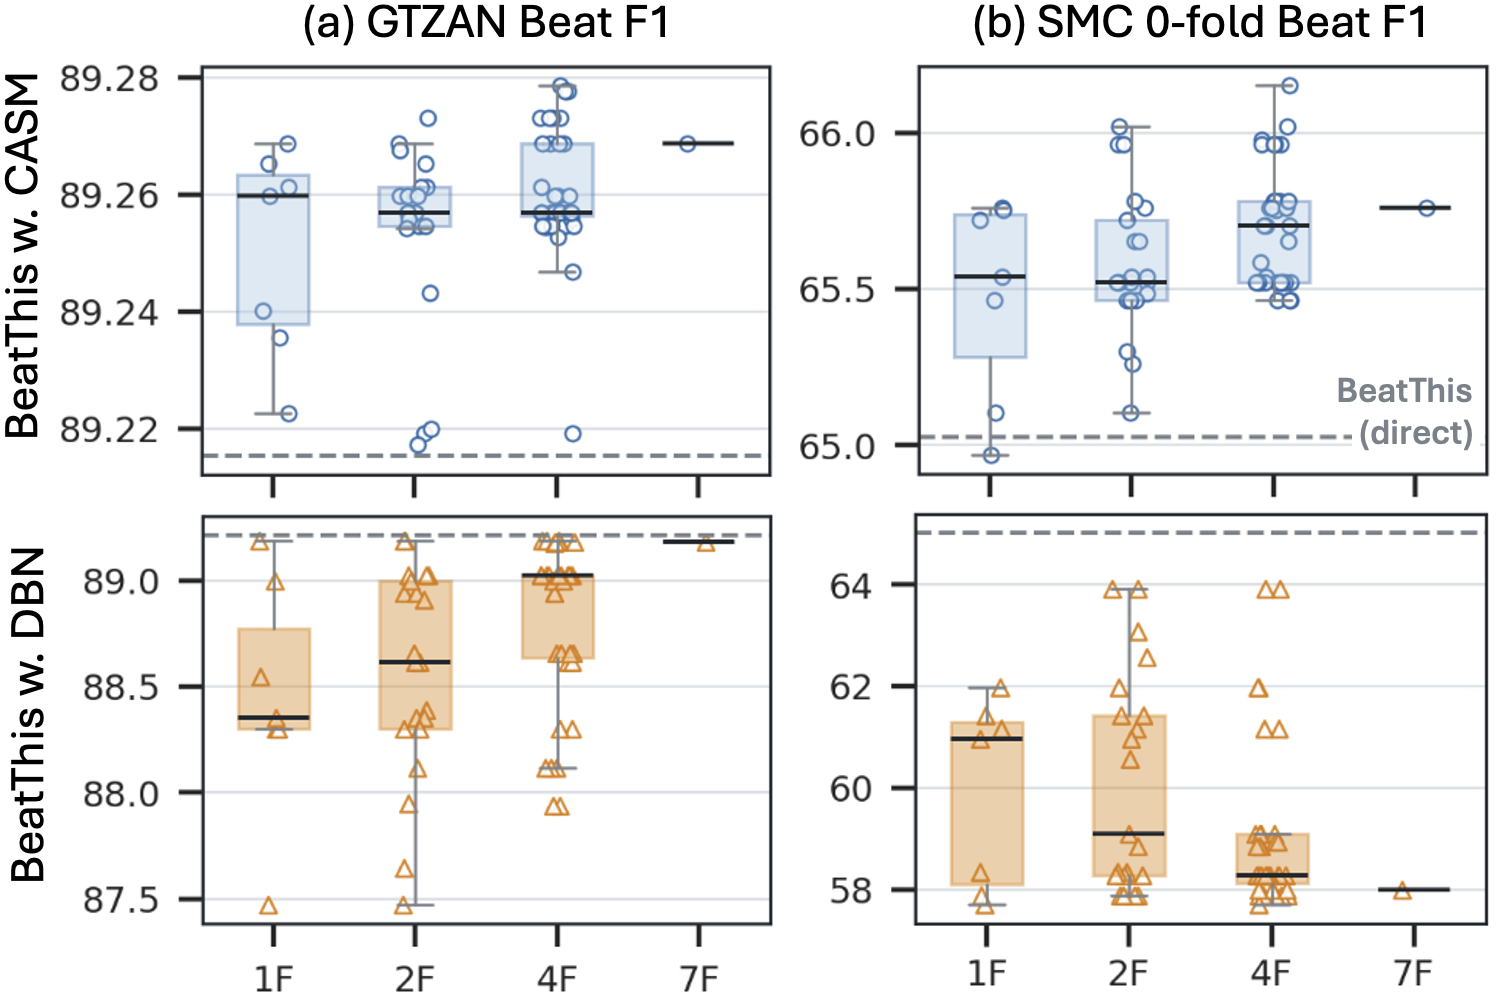
\includegraphics[width=0.9\columnwidth]{figures/p2.jpg}
\caption{Sensitivity to calibration data for CASM and DBN. Each point corresponds to a decoder configuration selected from one of the $7/21/35$ exhaustive 1-/2-/4-fold subsets of SMC folds 1--7 and evaluated on fixed SMC-fold-0 and GTZAN panels; 7F is a single configuration. Boxes are descriptive because calibration subsets overlap, and dashed lines show Direct performance.}
\label{fig:calibration-scale}
\end{center}
\end{figure}
\vspace{-3pt}
Fig.~\ref{fig:calibration-scale} shows a clear difference in calibration behaviour. CASM remains tightly clustered across fold combinations, and its central performance improves consistently as more calibration folds are used on both the held-out SMC panel and GTZAN. In contrast, DBN exhibits much wider variation across calibration subsets, and the trends on SMC and GTZAN do not move together: configurations favoured by one panel can transfer poorly to the other. This cross-dataset disagreement is consistent with stronger calibration-set over-specialisation in the fixed DBN parameterisation. The 7F CASM setting used in the main tables is therefore supported by the full available calibration pool rather than selected from a favourable smaller-fold combination.

\section{Conclusion and Future Work}
\label{sec:concl}

CASM revisits structured beat decoding as an inductive bias conditioned on each input, not as a return to a fixed global grid. It joins activation-supported events with locally centred segment potentials and deliberately relaxes those potentials when periodic evidence is ambiguous. Once globally calibrated, the same deterministic module runs without upstream retraining, user annotation, or per-track tempo and meter settings. Current evidence supports a conservative F1--continuity alternative to Direct and DBN decoding, not universal dominance. The next version should use strict nested or leave-one-dataset-out calibration, matched tempo-support baselines, PLPDP and mechanism ablations, and explicit safeguard statistics. Multi-hypothesis period paths, causal decoding, and a differentiable duration layer are natural extensions, as is evaluation on every recent tracker that releases compatible activations.

\textbf{Acknowledgments.}
The computational resources are supported by SongShan Lake HPC
Center (SSL-HPC) at Great Bay University.

\bibliographystyle{IEEEbib}
\bibliography{casm}

\end{document}